



%\{Some Properties of Batch-Normalized Networks}
\section{Some other normalization methods in deep learning}
In this section, we will discuss some other normalization methods in deep neural networks.
We will try to propose a general framework for  these normalization methods which also include the batch normalization.

\subsection{A general framework for normalization in deep neural networks}
Following the idea and notation in the previous section. We consider the data set as
\begin{equation}\label{eq:trainingdata1}
(X,Y) := \{x^i, y^i\}_{i=1}^N.
\end{equation}
For simplicity, here we just focus on the normalization operator during one hidden layer like:
\begin{equation}
\begin{cases}
z &= Wx + b,\\
y &= \sigma(z) 
\end{cases}
\end{equation}
where 
\begin{equation}
x \in \mathbb{R}^d, \quad W \in \mathbb{R}^{d\times n}
\end{equation}
Based on these setup, we give the next general framework for normalization in deep neural network as
\begin{equation}\label{eq:norm-h}
\begin{cases}
z &= Wx + b,\\
\tilde  z &= h(z),\\
y &= \sigma(\tilde z).
\end{cases}
\end{equation}
Here $h: \mathbb{R}^{n} \mapsto \mathbb{R}^n$ has a general form as
$$
h(z) = \gamma_N \frac{z - \mu_N}{\sigma_N} + \beta_N,
$$
where $\gamma_N, \mu_N, \sigma_N, \beta_N \in \mathbb{R}^n$, and all operation will be applied element-wise.

For the above formulation, we have the next relation immediately.
\begin{itemize}
	\item If $h = {\rm id}$, it recover the original DNN models.
	\item If $h(z) = {\rm BN}_{X}(z)$, then it recovers the BN method with the ``modified" SGD training strategy.
\end{itemize}


\subsection{Some example of normalization in DNN}
Then, we will show that, they are many existing normalization methods which can be formulated with 
special choice of $h(\cdot)$.

\paragraph{Layer Normalization (LN)}
The idea behind layer normalization is quite similar to batch normalization.
Batch normalization requires to do average or expectation with respect to the data direction.
For example, in batch normalization we have
$$
\mu_{BN} = \mu_X = \sum_{i=1}^N z(x^i) = \mathbb{E}_{s \sim X}[ z(x)].
$$
What layer normalization does is to take mean, (average, expectation) in the neuron (feature, space) direction.
That is to say, we can take those parameters in $h(\cdot)$ as:
\begin{equation}\label{eq:LN-mu}
\mu_{LN} = \frac{1}{n}\sum_{k=1}^n z_k, \quad \sigma_{LN}=\sqrt{\frac{1}{n}\sum_{k=1}^{n}(z_k-\mu_{LN})}.
\end{equation}
Here $\mu_{LN}  ,  \sigma_{LN} \in \mathbb{R}$, so we may put 
$$ 
\mu_{LN} \bm 1,  \sigma_{LN} \bm 1 \in \mathbb{R}^n,
$$
with 
$$
\bm 1 = (1, \cdots, 1) \in \mathbb{R}^n,
$$
for rigorous statement. 
With the similar situation in batch normalization, we can take $\gamma_{LN}, \beta_{BN} \in \mathbb{R}^n$. This means that
we can also remove the bias $b$ in original DNN.
Thus to say, we have the layer normalization transformation as:
\begin{equation}\label{eq:LN-h}
h_{LN}(z) = \gamma_{LN} \frac{z - \mu_{LN}\bm 1}{\sigma_{LN} \bm 1} + \beta_{LN}.
\end{equation}
More details of this normalization can be found in \cite{ba2016layer} by G. Hinton for RNN models.


\paragraph{Weight Normalization (WN)}
Weight normalization  normalizes the 
row norm of the matrix  $W$ in fully connected layer instead of 
the output $z$.
To normalize $W_k$, i.e. keep the 2-norm of $W_k$ to $1$, we may 
have a weight normalization transformation as
$$
[{\rm WN}(z(x)) ]_k= \gamma_k \frac{W_k \cdot x}{\|W_k\|_{2}} + b_k.
$$
This is a little different from the $h(\cdot)$ above, but we can still recover this
by choosing those parameters carefully.
Here, in weight normalization, we can take 
\begin{equation}
\mu_{WN} = b,\quad  \sigma_{WN} = \left( \|W_1\|_{2}, \cdots \|W_n\|_{2}\right),\quad \beta_{WN} = b,
\end{equation}
with $\gamma_{WN}$ free.
More details can be found in \cite{salimans2016weight}.

\paragraph{Cosine Normalization (CN)}
Cosine normalization normalizes both $W_k$ and the data $z$. 
It can be shown as
$$
[{\rm CN}(z(x)) ]_k= \gamma_k \frac{(W_k, b_k) \cdot (x,1) }{\|(W_k,b_k)\|_{2} \|(x,1)\|_{2}}.
$$
We can also recover this by choosing those parameters carefully.
Here, in cosine normalization, we can take 
\begin{equation}
\mu_{CN} = 0,\quad  \sigma_{WN} =  \|(x,1)\|_{2}\left(\|(W_1,b_1)\|_{2}, \cdots \|(W_n,b_n)\|_{2}\right),\quad \beta_{WN} = 0,
\end{equation}
with $\gamma_{WN}$ free.
More details can be found in \cite{luo2018cosine}.

\paragraph{Spectral Normalization (SN)}
The original idea in spectral normalization is to control the ``robustness'' of the deep neural networks.
Thus to say, if you have a small perturbation in input data, the output should 
also keep stable.
For ReLU DNN, the ``robustness'' means the Lipschitz  continuity because of the regularity of ReLU.

One hidden layer as example, 
\begin{equation}
\| \sigma(Wx + b) - \sigma(W(x+\Delta x) + b)\|_2 \le \|W\Delta x\|_2,
\end{equation}
this means that the Lipschitz constant for $\sigma(Wx+b)$ equals to $\|W\|_2 = \sigma (W)$ where
\begin{equation}
\sigma(W)=\max_{x\neq0}\frac{\|Wx\|_2}{\|x\|_2}.
\end{equation}
For ReLU DNN case,
$$
\|f^J(x;\Theta)\|_{\rm Lip} \le \Pi_{\ell=0}^J \sigma(W).
$$
Spectral normalization devotes to normalize the$ \|f^J(x;\Theta)\|_{\rm Lip} $ to be 1.
This can hold if 
$$
\sigma (W^\ell) = 1, \quad \forall \ell = 0:J.
$$
So, it is natural to add the next normalization 
$$
{\rm SN}(z(x)) = \frac{ Wx }{\sigma(W)} + b.
$$
Then, it can be recovered from $h(\cdot)$ simply by choosing
\begin{equation}
\mu_{CN} = b,\quad  \sigma_{CN} =  \sigma(W),\quad \gamma_{CN} = 1, \quad \beta_{CN} = b.
\end{equation}

\begin{remark}
Generally speaking, $\sigma (W)$ is difficult to take gradient. They use some trick in the paper \cite{miyato2018spectral}.
\end{remark}


%The authors of SN argues that an advantage of smaller $\sigma(W)$ is that $Wx$ is less sensitive to the perturbation $\xi$ on $x$, because
%\begin{equation}
%	\frac{\|(W(x+\xi)+b)-(Wx+b)\|}{\|\xi\|}=\frac{\|W\xi\|}{\|\xi\|}\leq\sigma(W).
%\end{equation}
%$\sigma(W)$ is thus added to the loss function, and gives
%\begin{equation}
%	L_\text{SN}(X)=\frac{1}{m}\sum_{i=1}^m\|f(x_i)-y_i\|_2^2+\frac{\lambda}{2}\sum_{l=1}^{n_L}\sigma(W_l)^2.
%\end{equation}


\paragraph{Group Normalization (GN)}
This method is proposed by Kaiming He, 
for the limitation of batch normalization with
\begin{itemize}
	\item If mini-batch is big, computation coast.
	\item if mini-batch is small, result is poor.
\end{itemize}
The idea is that, the feature in channel dimension (neuron dimension) should
group each together if they share similar features. That is to say, for example,
$$
(z_1, z_2, \cdots, z_n) = \left( (z_{1}, \cdots, z_{g}), (z_{g+1}, \cdots, z_{2g}), \cdots, (z_{n-g+1}, z_{n})\right),
$$
and in each group 
$$
(z_{kg+1}, \cdots, z_{(k+1)g}), \quad k = 0:\frac{n}{g}-1,
$$
should share the similar distribution which means we should take average just in this group.
Thus to say, we have the next formula for $\mu_{GN}$ and $\sigma_{GN}$,
\begin{equation}\label{eq:GN-mu}
\mu_{GN} = (\mu_1 \bm 1_{g}, \cdots, \mu_{\frac{n}{g}} \bm 1_g), \quad \sigma_{GN} = (\sigma_1 \bm 1_{g}, \cdots, \sigma_{\frac{n}{g}} \bm 1_g),
\end{equation}
with 
$$
\mu_{k} = \frac{1}{g}\sum_{i = (k-1)g+1}^{kg} z_i, \quad \sigma_k = \sqrt{\frac{1}{g} \sum_{i = (k-1)g+1}^{kg}(z_i - \mu_k)^2}.
$$

\begin{figure*}[!htb]
	\centering
	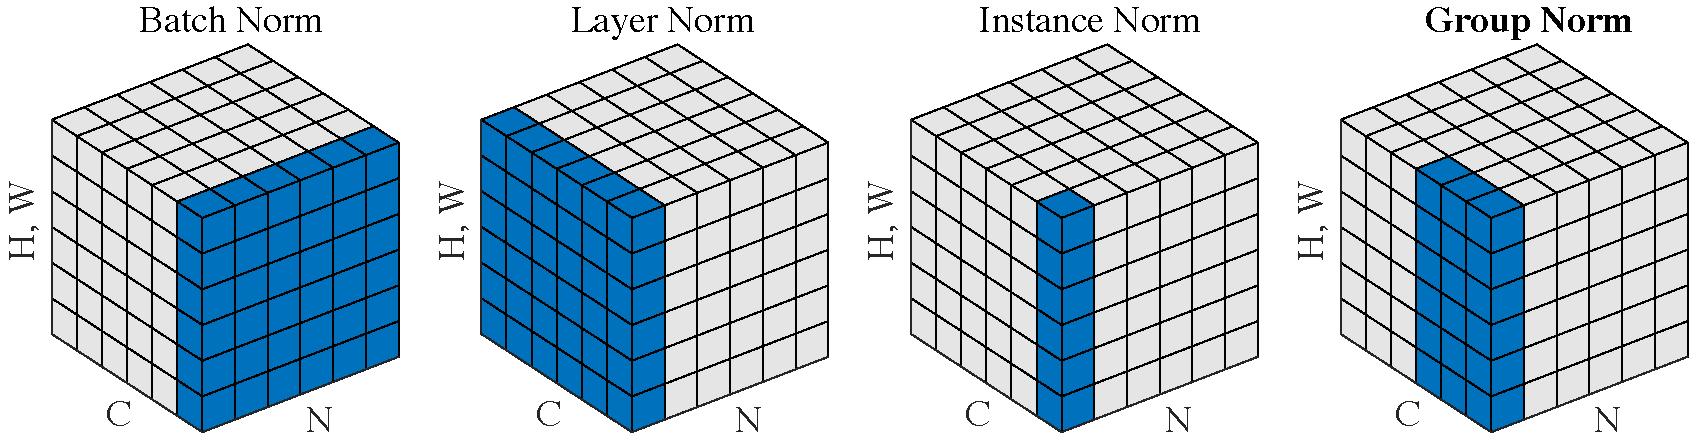
\includegraphics[width=.72\linewidth]{GN_all_norms}
	\vspace{.5em}
	\caption{\textbf{Normalization methods}. Each subplot shows a feature map tensor, with $N$ as the batch axis, $C$ as the channel axis, and $(H, W)$ as the spatial axes.
		The pixels in blue are normalized by the same mean and variance, computed by aggregating the values of these pixels.
	}
	\label{fig:all_norms}
	\vspace{-.5em}
\end{figure*}
More details can be found in \cite{wu2018group}.




\section{Example: numerical results for different normalizations}
The methods are tested with a two-hidden-layer fully connected neural network, with Adam optimizer of learning rate 0.01.

The two hidden layers are both applied the same normalization methods. The first hidden layer has 128 neurons, and the second 64 neurons.

The dataset is MNIST. The training batch size is 64.

\begin{figure}[H]
	\center
	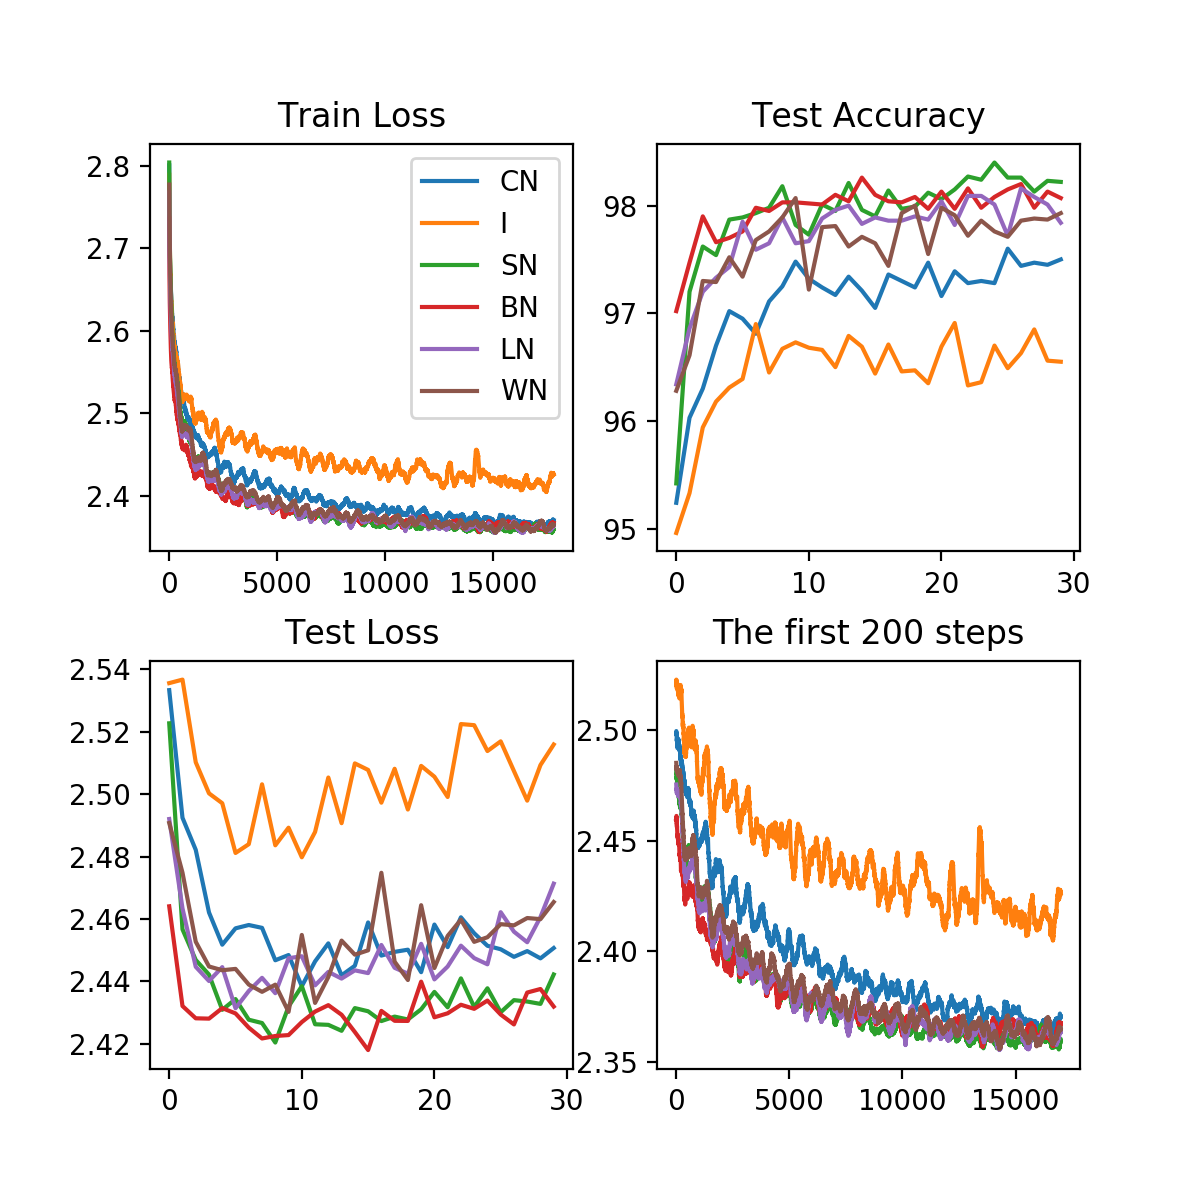
\includegraphics[width=0.8\textwidth]{Normal_res1.png}
	\caption{Comparison between different normalization methods. I means identity, i.e. without any normalization.}
\end{figure}

\begin{figure}[H]
	\center
	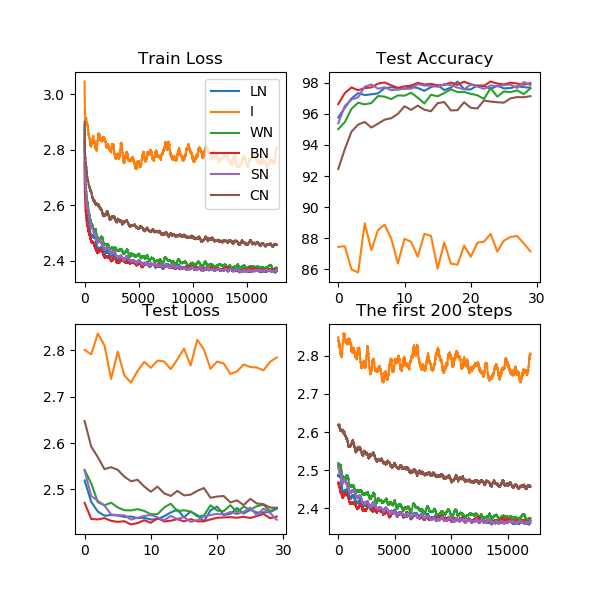
\includegraphics[width=0.8\textwidth]{Normal_res2.png}
	\caption{Use ReLU as activation.}
\end{figure}